\documentclass[journal]{IEEEtran}

%\documentclass[10pt]{beamer}
%\usepackage[left=1in,top=1in,right=1in,bottom=1in]{geometry}
\newcommand*{\authorfont}{\fontfamily{phv}\selectfont}
\usepackage{lmodern}

\usepackage{animate}
\usepackage[T1]{fontenc}
\usepackage{blindtext}
\usepackage{graphicx}
\usepackage{booktabs} % For formal tables
\usepackage{amsbsy}
\usepackage[ruled]{algorithm2e} % For algorithms
\usepackage{multirow}
\usepackage{amssymb}
\usepackage{amsmath}
\usepackage{tikz}
\usepackage[utf8]{inputenc}
\usepackage[english]{babel}
\usepackage{color}
\usepackage{soul}
\usepackage{fancyhdr}
\usepackage{float}
\usepackage{hyperref} 

\usepackage{amsthm}
\usepackage{mathtools}
\usepackage{xcolor}
\usepackage{pgfplots}
\usepackage{pdfpages}

\usepackage{xcolor}
\usepackage{listings}

\usepackage{xparse}

\NewDocumentCommand{\codeword}{v}{%
\texttt{\textcolor{blue}{#1}}%
}


\usepackage{verbatim}
\DeclarePairedDelimiter{\ceil}{\lceil}{\rceil}
\makeatletter
\def\thm@space@setup{%
  \thm@preskip=8pt plus 2pt minus 4pt
  \thm@postskip=\thm@preskip
}
\makeatother


%\newtheorem{theorem}{Theorem}[section]
%\newtheorem{corollary}{Corollary}[theorem]
%\newtheorem{lemma}[theorem]{Lemma}
%\newtheorem{definition}{Definition}[section]
\usetikzlibrary{automata, positioning}
\renewcommand{\algorithmcfname}{ALGORITHM}
\providecommand{\tightlist}{%
  \setlength{\itemsep}{0pt}\setlength{\parskip}{0pt}}

\fancypagestyle{firstpage}{% Page style for first page
  \fancyhf{}% Clear header/footer
  \renewcommand{\headrulewidth}{0.0pt}% Header rule
  \renewcommand{\footrulewidth}{0.0pt}% Footer rule
  \fancyhead[R]{\footnotesize{\thepage}}
  % Header
  %\fancyfoot[C]{-~\thepage~-}% Footer
}


\usepackage{setspace}


% set default figure placement to htbp

\usepackage{hyperref}
\usepackage{amsmath,tabu}
\usepackage{type1cm}

% add some other packages ----------

% \usepackage{multicol}
% This should regulate where figures float
% See: https://tex.stackexchange.com/questions/2275/keeping-tables-figures-close-to-where-they-are-mentioned
\usepackage[section]{placeins}



\begin{document}
\onecolumn
% \pagenumbering{arabic}% resets `page` counter to 1 
%
% \maketitle

% \textbf{----------------------------------------}

% \textbf{Network SLEC DP Definitions}

% Assume that we have $r$ racks, and each rack has $v$ disks. We still have $n=k+m$ where k is the data chunks and m is the parity chunks. To differentiate the difference between network speed and local disk speed, we introduce $S_{net_R}$ and $S_{net_W}$ as the network read write speed.

% We also assume that there is only single enclosure per rack, as there is no implementation that differentiate rack and enclosure in \verb|mlec-sim|. Therefore, Network SLEC DP ensures that each rack will contain at most 1 chunk out of a $n=k+m$ stripe.\\


% \textbf{Repair Rate of single damaged stripes in Network SLEC DP}

% When there is a single drive failure, we know that for all the impacted stripes, the other $n-1$ chunks are going to reside on other racks. Therefore, the number of disks that might contain stripes affected by this single failure is $(r-1)*v$, and these disks are going to participate in the repair of the failed disk.

% Therefore we have the following conditions
% \begin{itemize}
%     \item We have declustered parallelism of $(r-1)*v$
%     \item We read $\mathcal{CAP}(n-1)$ amount of data
%     \item We write $\mathcal{CAP}*1$ amount of data
% \end{itemize}

% We can then calculate the duration as the sum of duration to read and write as following. We assume that $S_{net_W}=S_{net_R}=S_{net}$
% \begin{equation*}
%     Duration=\frac{(n-1)\mathcal{CAP}}{(r-1)*v*S_{net}}+\frac{\mathcal{CAP}}{(r-1)*v*S_{net}}=\frac{n\mathcal{CAP}}{(r-1)*v*S_{net}}
% \end{equation*}

% Comparing with the standard repair rate of RAID which is $\mu=\frac{\mathcal{CAP}}{S_{disk}}$, we can get
% \begin{equation*}
%     \mu_1=\mu\frac{nS_{disk}}{(r-1)*v*S_{net}}
% \end{equation*}

\textbf{SLEC Priority Percent Calculation [WIP]}

\textbf{----------------------------------------}

\textbf{Discussion on General Ideas}

The math note is an expansion on the combinatorics calculation implemented in the MLEC sim's flat DP mode. The concept is simple - when we have a disk failure, we are interested in how many data on the drive (priority percent) belongs to the disk's priority and then we can calculate the time needed for repair in relation to normal RAID. Knowing the repair time in relation to normal RAID, we can then calculate the MTTDL of network SLEC DP in relation to normal RAID and mathematically calculate the number of nines for network SLEC DP durability.\

\hspace*{1cm}

\textbf{Notations}

\begin{itemize}
  \item $r$: number of racks
  \item $B$: number of disks per rack
  \item $k$: number of data chunks
  \item $m$: number of parity chunks
  \item $p$: the current priority of the disk
  \item $n$: stripe width $(k+m)$
  \item $f$: total number of failed disk
  \item $f_s$: number of failures in the stripe (number of disks that we need to repair)
  \item $f_{r_[i]}$: number of failures in the rack, with parameter $[i]$ indicating which rack the variable is referring to
  \item $\mathcal{CAP}$: capacity of the disk
  \item $S_{net_W}=S_{net_R}=S_{net}$: speed of network IO
  \item $S_{disk_W}=S_{disk_R}=S_{disk}$: speed of disk
\end{itemize}

\hspace*{1cm}

\textbf{Discussion on Speed Bottleneck}

For the sake of simplicity for discussion, we currently assume that the network bandwidth $S_{net}=\infty$, so that we only consider $S_{disk}$ during repair operations. In the future we will make more indepth analysis of the network bandwidth's impact on repair speed.

\hspace*{1cm}

\textbf{Discussion on Parallelism}

Due to the constraint that network SLEC DP places on chunk placement, when there is failure, we read from one node per rack for all other racks ($k$ in total). We use the following notation
\begin{itemize}
  \item $f$: total number of failed disk
\end{itemize}

\begin{equation*}
  \text{read parallelism}=(r-f_s)B
\end{equation*}

When writing the reconstructed chunk to the \textit{virtual reserved space}, we still want to utilize all of the virutal reserved spaces on all the surviving disks to maximize reconstruction. Therefore,
\begin{equation*}
  \text{write parallelism}=rB-f
\end{equation*}

\hspace*{1cm}

\textbf{Discussion on Priority Percent Calculation for Plain DP}

We can see from the general discussion that we are interested in knowing what percentage of data on the failed disk belongs to which priority, and repair them at different speeds/priority. The following rough equation is how the calculation is carried out in plain DP. We first want to know the number of stripes that are in the degraded state (has at least one failed chunks). Therefore, we select $(n-1)$ drives from all the drives $(\text{good\_num}+\text{fail\_num}-1)$ (minus 1 for at least one failure). The total number of stripes in the degraded state is
\begin{equation*}
  \text{number of impacted stripes}=ncr(\text{good\_num}+\text{fail\_num}-1, n-1)
\end{equation*}

We then want to calculate how many stripes are of the current priority. We first select the surviving drives in the stripe from all the surviving drives.
\begin{equation*}
  \text{all possible surviving chunks}=ncr(\text{good\_num}, (n-p))
\end{equation*}

Then we select all the failed chunks out of failed drives. Note that since we have already included the \textit{at least one} failure in the total affected stripes calculation, we need to make adjustment here
\begin{equation*}
  \text{all possible failed chunks}=ncr(\text{fail\_num-1}, p-1)
\end{equation*}

Combining the three equations above, we can get the priority percentage calculation for \textbf{plain DP} as follows
\begin{equation*}
  \text{prio percent}=\frac{\text{possible failed chunks}*\text{possible surviving chunks}}{\text{affected stripes}}=\frac{ncr(\text{good\_num}, (n-p))*ncr(\text{fail\_num-1}, p-1)}{ncr(\text{good\_num}+\text{fail\_num}-1, n-1)}
\end{equation*}

\hspace*{1cm}

\textbf{Discussion on Priority Percent Calculation for SLEC network DP}

Working on finding a good looking model. See enumerated cases below.

\hspace*{1cm}

% For priority percent calculation of SLEC network DP, we are going to follow a similar concept, but make adjustments according to the constraint of one chunk per rack placement. Due to this constraint, we can see that
% \begin{itemize}
%   \item fail\_num should not be the total number of failed disks, but rather the number of failed disks in the stripe
%   \item good\_num should not be the total number of surviving disks, but rather the number of surviving drives on unimpacted racks (stripe level)
%   \item note that for the denominator, we still use $ncr(s+f-1, n-1)$ instead of $ncr(s+f_s-1, n-1)$ because we are calculating all the degraded stripes
% \end{itemize}

% Given these two modifications, the priority percent calculation becomes
% \begin{equation*}
%   \text{good\_num(SLEC)}=s=\sum_{\substack{i=0 \\ i\not\subset \text{impacted racks}}}^{r} (B-f_{r_i})
% \end{equation*}
% \begin{equation*}
%   \text{prio percent}==\frac{ncr(s, (n-p))*ncr(f_s-1, p-1)}{ncr(s+f-1, n-1)}
% \end{equation*}

% \hspace*{1cm}

\textbf{Enumerate Some Cases}

\section{When there is a single failure [distinct rack], this means that}
\begin{itemize}
  \item All the affected stripes must not have another drive on the same rack due to the placement constraint
  \item The number of failed drive is 1 and has priority of 1
  \item The percent of stripes of priority 1 out of all the affected stripes is
\end{itemize}

\begin{equation*}
  \text{prio percent}=\frac{ncr(r-1,n-1)B^{n-1}}{ncr(r-1,n-1)B^{n-1}}=1
\end{equation*}

Explaning the equation: for the numerator, we know that there is a single failed disk. Therefore, we select the surviving chunks $(n-1)$ of stripes from the surviving \textbf{racks} (not disk because of the placement constraint) $(r-1)$. However, we also have the choice of $B$ disks in each of the surviving racks. Therefore, we add the multiplier of $B^{r-1}$. For the denomenator, we have the total number of stripes that have at least one failed chunk. Therefore, the equation is identical to the numerator.

% We can see that in terms of parallel repair of DP, we can only read/write from and to the disks that do not reside on the same rack. Therefore we will have the parallelism as $(r-1)B$. 

% The amplification is reading from $k$ chunks and writing to $f_s$(in this case 1) chunk.

% Therefore the time needed for repair calculation is as follows
% \begin{equation*}
%   \frac{\mathcal{CAP}(k+f_s)}{S_{net}(r-1)B/f_s}
% \end{equation*}

\section{When there are two failures [same rack], this means that the \textbf{priority 1 stripes} }
\begin{itemize}
  \item We will \textbf{only} have priority 1 stripes because there cannot be any stripes that contains both of the failed disk on the same rack. This means that the percent of priority 1 stripe out of all the affected stripe should be 1.
  \item The percent of stripes of priority 1 out of all the affected stripes is
\end{itemize}

\begin{equation*}
  \text{prio percent}=\frac{ncr(r-1, n-1)B^{n-1}}{ncr(r-1, n-1)B^{n-1}}=1
\end{equation*}

\section{When there are two failures [distinct rack], this means that \textbf{priority 1 stripe}}
\begin{itemize}
  \item For the numerator, there are two conditions.
  \begin{itemize}
    \item stripes that have chunks sitting on both of the impacted racks (however does not contain both failed disk).
    \item stripes that have the failed chunk sitting on either of the impacted chunks.
  \end{itemize}
  \item The percent of stripes of priority 1 out of all the affected stripes is
\end{itemize}

\begin{equation*}
  \text{prio percent}=\frac{ncr(r-2,n-2)B^{n-2}(B-1)+ncr(r-2,n-1)B^{n-1}}{ncr(r-1,n-1)B^{n-1}}=\frac{B-1}{B}\frac{n-1}{r-1}+\frac{r-n}{r-1}
\end{equation*}

Using an example of $r=10,B=10,n=9$, we can see that the priority percent would be
\begin{equation*}
  \text{prio percent}=\frac{ncr(8,7)*10^7*9+ncr(8,8)*10^8}{ncr(9,8)*10^8}=\frac{82}{90}
\end{equation*}

\section{When there are two failures [distinct rack], this means that \textbf{priority 2 stripe}}
\begin{itemize}
  \item This means that all the priority 2 stripes contains both of the failed disks
  \item The percent of priority 2 stripes out of all the affected stripe is
\end{itemize}

\begin{equation*}
  \text{prio percent}=\frac{ncr(r-2,n-2)B^{n-2}}{ncr(r-1,n-1)B^{n-1}}=\frac{1}{B}\frac{n-1}{r-1}
\end{equation*}

Using the example of $r=10,B=10,n=9$, we can see that the priority percent would be
\begin{equation*}
  \text{prio percent}=\frac{ncr(8,7)*10^7}{ncr(9,8)*10^8}=\frac{8}{90}
\end{equation*}

We can see that this prio percent, combined with the prio percent of priority 1 stripes, addes up to 1. Which means that our model is correct.

\section{When there are three failures [same rack], this means that \textbf{priority 1 stripes}}
\begin{itemize}
  \item There will still be only priority 1 stripes
  \item This then makes the formula identical to single failure priority percent calculation
\end{itemize}

\begin{equation*}
  \text{prio percent}=\frac{ncr(r-1, n-1)B^{n-1}}{ncr(r-1, n-1)B^{n-1}}=1
\end{equation*}

\section{When there are three failures [1, 2]}

This graph shows an example of the failure pattern.
\begin{figure}[H]
  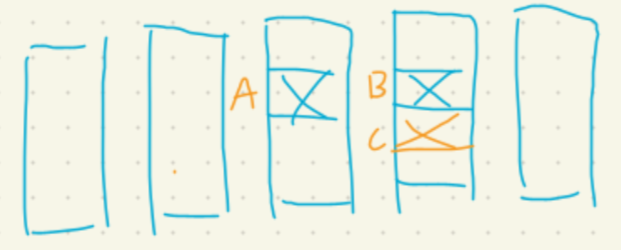
\includegraphics{img/3-1-2.png}
  \centering
\end{figure}
As we can see, due to the asymmetrical layout, we would have to discuss priority percent for each drive.

\subsection*{For priority 1 stripes on disk A}

\begin{itemize}
  \item It can either include a chunk on the rack with two failures, or only include chunks on unimpacted racks
  \item Therefore, the percentage of priority 1 stripes out of all the stripes that are impacted by disk A is
\end{itemize}

\begin{equation*}
  \text{prio percent}=\frac{ncr(r-2,n-2)B^{n-2}(B-2)+ncr(r-2,n-1)B^{n-1}}{ncr(r-1,n-1)B^{n-1}}=\frac{n-1}{r-1}\frac{B-2}{B}+\frac{r-n}{r-1}
\end{equation*}

\subsection*{For priority 2 stripes on disk A}
\begin{itemize}
  \item It can include either disk B or C as the second failed chunk, and it has to have failed chunks sitting on both of the rack.
  \item Therefore, the percentage of priority 2 stripes out of all the stripes that are impacted by disk A is
\end{itemize}

\begin{equation*}
  \text{prio percent}=\frac{ncr(r-2,n-2)B^{n-2}*2}{ncr(r-1,n-1)B^{n-1}}=\frac{n-1}{r-1}\frac{2}{B}
\end{equation*}

\subsection*{For priority 1 stripes on disk B/C}
\begin{itemize}
  \item It can include a chunk on rack of disk A, or have all other chunks sitting on unimpacted racks
  \item Therefore, the percentage of priority 1 stripes out of all the stripes that are impacted by disk B is
\end{itemize}

\begin{equation*}
  \text{prio percent}=\frac{ncr(r-2,n-2)B^{n-2}(B-1)+ncr(r-2,n-1)B^{n-1}}{ncr(r-1,n-1)B^{n-1}}=\frac{n-1}{r-1}\frac{B-1}{B}+\frac{r-n}{r-1}
\end{equation*}

\subsection*{For priority 2 stripes on disk B/C}
\begin{itemize}
  \item It has to include disk A
  \item Therefore, the percentage of priority 2 stripe sout of all the stripes that are impacted by disk B is
\end{itemize}

\begin{equation*}
  \text{prio percent}=\frac{ncr(r-2,n-2)B^{n-2}}{ncr(r-1,n-1)B^{n-1}}=\frac{n-1}{r-1}\frac{1}{B}
\end{equation*}

\section{When there are three failures [distinct rack], this means \textbf{priority 1 stripes}}
\begin{itemize}
  \item We have three scenarios to select good ones out of
  \item \begin{itemize}
    \item All the other chunks are sitting on unimpacted racks
    \item One chunk is sitting on any of the other two impacted racks
    \item Two chunks are sitting on the other two impacted racks
  \end{itemize}
  \item Therefore, the percentage of priority 1 stripes out of all the stripes that are impacted by one of the failed disks is
\end{itemize}

\begin{equation*}
  \begin{split}
    \text{prio percent} 
    & =\frac{ncr(r-3,n-1)B^{n-1}+ncr(r-3,n-2)B^{n-2}(B-1)+ncr(r-3,n-3)B^{n-3}(B-1)^2}{ncr(r-1,n-1)B^{n-1}} \\
    & =\frac{(r-n)(r-n-1)}{(r-1)(r-2)}+2\frac{(r-n)(n-1)}{(r-1)(r-2)}\frac{B(B-1)}{B^2}+\frac{(n-1)(n-2)}{(r-1)(r-2)}\frac{(B-1)^2}{B^2}
  \end{split}
\end{equation*}

\section{When there are three failures [distinct] rack, this means \textbf{priority 2 stripes}}
\begin{itemize}
  \item Note that in all the previous priority percent calculation, we only select the good chunks out of the surviving disks (given the rack constraint). However, note that we derive our intuition from the priority percent calculation for flat DP, which involves selecting failed chunks out of all the failed disks as well. This was not needed in all the previous calculations because it would all result in 1, but it starts to matter now.
  \item There are two scenarios we need to consider
  \item \begin{itemize}
    \item Stripe containing two failed chunks on two of the impacted racks, and all other chunks reside on unimpacted racks
    \item Stripe containing two failed chunks on two of the impacted racks, and one of the surviving chunk reside on the other impacted rack
  \end{itemize}
  \item For each of the above scenario, we can see that we have $ncr(2,1)=2$ ways of choosing the two failed chunks out of the three failed disks.
  \item Therefore, the percentage of priority 2 stripes out of all the stripes that are impacted by one of the failed disks is
\end{itemize}

\begin{equation*}
  \begin{split}
    \text{prio percent}
    & =\frac{ncr(r-3,n-2)B^{n-2}ncr(2,1)+ncr(r-3,n-3)B^{n-3}(B-1)ncr(2,1)}{ncr(r-1,n-1)B^{n-1}}\\
    & =\frac{(r-n)(n-1)}{(r-1)(r-2)}\frac{2B}{B^2}+\frac{(n-1)(n-2)}{(r-1)(r-2)}\frac{2(B-1)}{B^2}
  \end{split}
\end{equation*}

\section{When there are three failures [distinct] rack, this means \textbf{priority 3 stripes}}
\begin{itemize}
  \item Have 3 failed chunks sitting on each of the impacted racks
  \item Therefore, the percentage of priority 3 stripes out of all the stripes that are impacted by one of the failed disks is
\end{itemize}

\begin{equation*}
  \text{prio percent}=\frac{ncr(r-3,n-3)B^{n-3}}{ncr(r-1,n-1)B^{n-1}}=\frac{(n-1)(n-2)}{(r-1)(r-2)}\frac{1}{B^2}
\end{equation*}

\section{When there are $\mathcal{N}$ failures, this means that priority $\mathcal{N}$ stripe}
\begin{equation*}
  \text{prio percent}=\frac{ncr(r-\mathcal{N},n-\mathcal{N})B^{n-\mathcal{N}}}{ncr(r-1,n-1)B^{n-1}}=\frac{1}{B^{\mathcal{N}-1}}\frac{\prod_{i=1}^{\mathcal{N}-1}(n-i)}{\prod_{i=1}^{\mathcal{N}-1}(r-i)}
\end{equation*}

\end{document}